% Fig. 1 teaser: full-width, set under the title by main.tex (\twocolumn[{...}]).
% Accepted design with current Table 1 results (2026-11-04): figures/Fig1/INDEX.md.
\begin{center}
\captionsetup{type=figure}
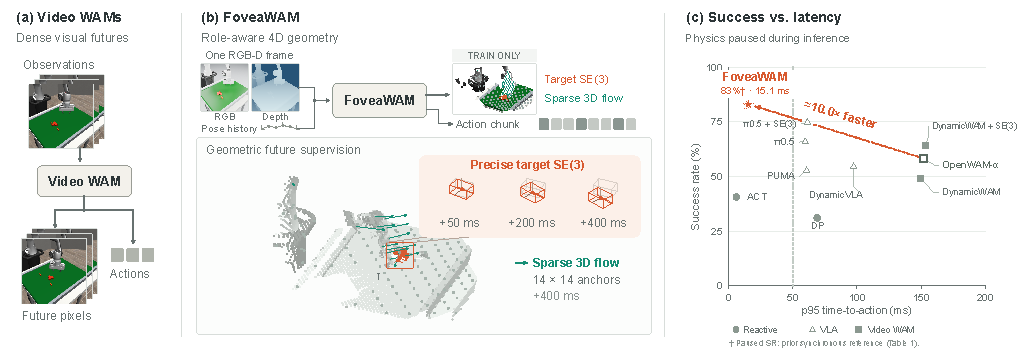
\includegraphics[width=\textwidth]{figures/Fig1/fig1.pdf}
\captionof{figure}{\textbf{\ours allocates prediction precision by task role.}
(a) Reference recordings illustrate dense video-future prediction and action outputs.
(b) One RGB-D frame and pose history condition \ours, with training-only target SE(3)
and sparse 3D flow supervision; action chunks are produced at deployment.
The RGB illustration is a Blender rendering of the recorded state; depth and point
clouds use recorded observations. Future geometry shows ground-truth supervision.
Flow is sampled on a
\cfgContextGrid{} grid; arrows show 400\,ms displacements enlarged $3\times$.
The lower pose glyphs show the target at $+50$, $+200$, and $+400$\,ms.
(c) Table~\ref{tab:main} Paused success (physics paused during inference) versus native
p95 time-to-action. The dashed line marks 50\,ms. The \ours star uses the reported
83\%$^{\dagger}$ and measured 15.1\,ms, giving $\approx10.0\times$ speedup over
OpenWAM-$\alpha$ (151.7\,ms). $^{\dagger}$The Paused value follows the prior
synchronous reference selected in Table~\ref{tab:main}.}
\label{fig:teaser}
\end{center}
